\documentclass[12pt]{article}
\usepackage[utf8]{inputenc}
\usepackage{graphicx}
\usepackage{amsmath}
%\usepackage[fceqn]{amsmath,amssymb}
\usepackage[bottom=2.0cm,top=2.0cm,left=2.5cm,right=2.5cm]{geometry}
\usepackage[portuges]{babel}
\usepackage{indentfirst}
\usepackage{wrapfig}
\usepackage{mathrsfs}
\usepackage{subcaption}
\usepackage{textcomp}
\usepackage[export]{adjustbox}
\usepackage{setspace}
\usepackage{stackengine}
\usepackage{hyperref}
\usepackage{listings}
\usepackage{xcolor}
\usepackage{float}
\usepackage{enumerate}  
\usepackage{enumitem}


% --- Configurações de espaçamento entre parágrafos ---
% A linha abaixo remove a indentação do parágrafo. 
% Para um melhor controle do espaço entre parágrafos, considere usar \usepackage{parskip}.
\setlength\parindent{0pt}

% --- Configurações do Hyperref ---
\hypersetup{colorlinks,citecolor=black,filecolor=black,linkcolor=black,urlcolor=black}

% --- Definição de cores para o código ---
\definecolor{mGreen}{rgb}{0,0.6,0}
\definecolor{mGray}{rgb}{0.5,0.5,0.5}
\definecolor{mPurple}{rgb}{0.58,0,0.82}
\definecolor{backgroundColour}{rgb}{0.95,0.95,0.92}

% --- Estilo para a listagem de código C ---
\lstdefinestyle{c}{
    %backgroundcolor=\color{backgroundColour},   
    %commentstyle=\color{mGreen},
    %keywordstyle=\color{magenta},
    %numberstyle=\tiny\color{mGray},
    %stringstyle=\color{mPurple},
    basicstyle=\footnotesize\ttfamily, % Adicionado \ttfamily para uma fonte monoespaçada
    breakatwhitespace=false,         
    breaklines=true,                 
    captionpos=b,                    
    keepspaces=true,                 
    numbers=left,                    
    numbersep=5pt,                   
    showspaces=false,                
    showstringspaces=false,
    showtabs=false,                  
    tabsize=2,
    language=C
}


\begin{document}

\begin{center}
    
\includegraphics[scale=0.25, valign=c]{ufersa-logo.png}
\end{center}
\begin{minipage}[c]{\textwidth}
\centering
\large{ {\bfseries UNIVERSIDADE FEDERAL RURAL DO SEMI-ÁRIDO - UFERSA} \\ {\bfseries DEPARTAMENTO DE ENGENHARIAS E TECNOLOGIA} \\ {\bfseries DISCIPLINA}: Laboratório de Algoritmos e Estrutura de Dados I \\ {\bfseries PROFESSOR:} George Felipe Fernandes Vieira\\ {\bfseries ALUNO:} Enthony Araujo de Oliveira }
\end{minipage}

\section*{Atividade 1 - Laboratório de Algoritmos e Estrutura de Dados I}

\textbf{Questão 1:} O que é e para que serve um ponteiro?
\\

\noindent\textbf{Solução:}

Ponteiros são variáveis que armazenam endereços na memória, eles são utilizados para manipulação eficiente da memória. 
\\

\textbf{Questão 2:} Declare uma variável e “printe” o valor dela e o seu endereço.
\\

\noindent\textbf{Solução:}
\begin{lstlisting}[style=c]
#include <stdio.h>

int main(){

    int idade = 22;

    printf("%d\n",idade);
    printf("%p\n", &idade);

    return 0;
}
\end{lstlisting}
Saída: 
\begin{figure}[h]
    \centering
    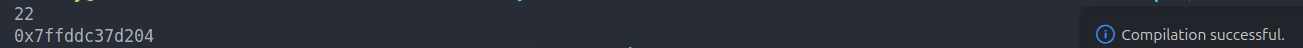
\includegraphics[width=1\linewidth]{images/2.png}
    \caption{Questão 2}
    \label{fig:placeholder}
\end{figure}
\\

\textbf{Questão 3:} Qual é a maneira correta de referenciar ch, assumindo que o endereço de ch
foi atribuído ao ponteiro indica?
\\

\noindent\textbf{Solução: }
\begin{lstlisting}[style=c]
#include <stdio.h>

int main(){
    
    char ch = 'A';
    char* indica;
    indica = &ch;

    printf("Valor de ch direto: %c\n", ch);
    printf("Valor de ch pelo ponteiro: %c\n",*indica);

    return 0;
}
\end{lstlisting}
\begin{figure}[h]
    \centering
    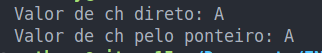
\includegraphics[width=0.5\linewidth]{images/3.png}
    \caption{Questão 3}
    \label{fig:placeholder}
\end{figure}
\\

\textbf{Questão 4:}Na expressão float *ptr; o que é do tipo float?
\\

\noindent\textbf{Solução:}
Na expressão o \textbf{float} não é uma variável, mas sim o valor para qual o ponteiro está apontando. 
\\

\textbf{Questão 5:}Como seria o output se eu desse “print” nas variáveis a seguir:
\begin{center}
    \begin{verbatim}
    int x = 68, y;
    int *p;
    p = &x;
    y = *p + 200;
    \end{verbatim}
\end{center}
\\

\noindent\textbf{Solução:}

\begin{figure}[h]
    \centering
    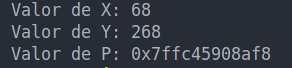
\includegraphics[width=0.5\linewidth]{images/5.png}
    \caption{Questão 5}
    \label{fig:placeholder}
\end{figure}
\\

\textbf{Questão 6: } Assumindo que queremos ler o valor de x, e o endereço de x foi atribuído a
px, a instrução seguinte é correta? Por que?
\begin{verbatim}
    scanf ( "%d", *px );
\end{verbatim}
\\

\noindent\textbf{Solução: }
A instrução não está correta. A função \textbf{scanf} precisa receber o endereço da variável onde vai guardar o valor.  
Se usamos \verb|&x|, passamos o endereço de \texttt{x}.  
Como \texttt{px} já guarda o endereço de \texttt{x}, podemos usar:
\[
\texttt{scanf("\%d", px);}
\]
O erro está em usar \verb|*px|, pois isso representa o conteúdo (valor de \texttt{x}), não seu endereço.  
Portanto, a instrução correta é:
\[
\texttt{scanf("\%d", px);}
\]
\\

\textbf{Questão 7:} Desenvolva uma função que receba como parâmetro os ponteiros de
dois vetores de 5 posições. O procedimento deverá imprimir na tela os
valores contidos nos dois vetores de forma crescente (Utilize ponteiros).
\\

\noindent\textbf{Solução:}
\begin{lstlisting}[style=c]
#include <stdio.h>

void imprime_vetor_crescente(int *v1, int *v2) {
    int i, menor, maior;

    menor = *v1;
    maior = *v1;
    for (i = 0; i < 5; i++) {
        if (*(v1 + i) < menor) menor = *(v1 + i);
        if (*(v1 + i) > maior) maior = *(v1 + i);
        if (*(v2 + i) < menor) menor = *(v2 + i);
        if (*(v2 + i) > maior) maior = *(v2 + i);
    }

    for (int val = menor; val <= maior; val++) {
        for (i = 0; i < 5; i++) {
            if (*(v1 + i) == val || *(v2 + i) == val) {
                printf("%d ", val);
            }
        }
    }
}

int main() {
    int v1[5] = {2, 5, 9, 8, 3};
    int v2[5] = {7, 4, 1, 10, 6};

    printf("Saida: ");
    imprime_vetor_crescente(v1, v2);

    return 0;
}
\end{lstlisting}

\begin{figure}[h]
    \centering
    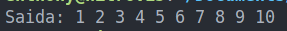
\includegraphics[width=0.5\linewidth]{images/7.png}
    \caption{Questão 7}
\end{figure}
\\

\textbf{Questão 8:} Assumindo que o endereço da variável x foi atribuído a um ponteiro px,
escreva uma expressão que não usa x e divida x por 3.
\\

\noindent\textbf{Solução:} 
\begin{lstlisting}[style=c]
#include <stdio.h>

int main() {
    int x = 9;        
    int *px = &x;     

    printf("Antes: x = %d\n", x);

    *px = *px / 3;

    printf("Depois: x = %d\n", x);

    return 0;
}
\end{lstlisting}
\begin{figure}[h]
    \centering
    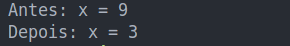
\includegraphics[width=0.5\linewidth]{images/9.png}
    \caption{Questão 8}
    \label{fig:placeholder}
\end{figure}
\\

\textbf{Questão 9:} Seja a seguinte sequência de instruções em um programa C:
\begin{verbatim}
    int *pti;
    int i = 10;
    pti = &i;
\end{verbatim}
    Qual afirmativa é falsa? Justifique a resposta
\begin{enumerate}[label=\Roman* -]
    \item pti armazena o endereço de i
    \item *pti é igual a 10
    \item ao se executar *pti = 20; i passará a ter o valor 20
    \item ao se alterar o valor de i, *pti será modificado
    \item pti é igual a 10
\end{enumerate}
\\

\noindent\textbf{Solução:}
Alternativa falsa é a \textbf{V}. Pois, pti é um ponteiro que armazena o endereço de i, portanto, seu valor é um endereço de memória, não o valor 10. O valor 10 está armazenado em i, e pode ser acessado via *pti, mas pti em si é um endereço.
\end{document}